\documentclass[11pt,letterpaper]{article}
\usepackage[T1]{fontenc}
\usepackage[utf8]{inputenc}
\usepackage{lmodern,microtype}
\usepackage[margin=0.91in,headheight=15pt]{geometry}
\usepackage{amsmath,amssymb,amsthm,mathtools}
\usepackage{booktabs,tabularx,longtable,array,multirow}
\usepackage{graphicx,caption,subcaption,float}
\usepackage[dvipsnames]{xcolor}
\usepackage{enumitem}
\usepackage{tikz}
\usetikzlibrary{arrows.meta,positioning,shapes.geometric,fit}
\usepackage{fancyhdr}
\usepackage{xurl}
\usepackage[colorlinks=true,linkcolor=NavyBlue,urlcolor=NavyBlue,citecolor=NavyBlue]{hyperref}
\usepackage[numbers,sort&compress]{natbib}
\usepackage{listings}
\definecolor{ink}{HTML}{1A2E40}
\definecolor{soft}{HTML}{EAF1F5}
\definecolor{muted}{HTML}{4C6073}
\setlength{\parskip}{0.42em}
\setlength{\parindent}{0pt}
\setlist{noitemsep,topsep=3pt}
\pagestyle{fancy}
\fancyhf{}
\fancyhead[L]{\small\textsc{FLOCK research notebook}}
\fancyhead[R]{\small October 2026}
\fancyfoot[C]{\thepage}
\newcommand{\observed}{\textsf{Source-verified}}
\newcommand{\partialresult}{\textsf{Partial log}}
\newcommand{\reported}{\textsf{Previously reported}}
\newcommand{\unverified}{\textsf{Unverified archive}}
\newcommand{\flock}{\textsc{flock}}
\newcommand{\dd}{\mathrm{d}}
\captionsetup{font=small,labelfont=bf}
\lstset{basicstyle=\ttfamily\footnotesize,breaklines=true,frame=single,columns=fullflexible,showstringspaces=false}
\hypersetup{pdftitle={FLOCK: Role-Specialized Exploration and Posterior Consolidation},pdfsubject={Research notebook; pilot simulation results and code provenance}}
\begin{document}
\begin{center}
{\Large\bfseries\color{ink} FLOCK: Role-Specialized Exploration\\[4pt] and Posterior Consolidation}\par
\vspace{7pt}
{\large A research notebook of designs, ablations, observed results, and failures}\par
\vspace{8pt}
{\small Working research record \textbullet\ October 2026 \textbullet\ Not a validated sampler or a submitted manuscript}
\end{center}
\vspace{6pt}
\begin{abstract}
We document an exploratory attempt to improve computational exploration of challenging posterior distributions by assigning different roles to multiple chains: aggressive scouts, local followers, novelty-seeking or geometry-guided pioneers, and a final posterior inference stage. We distinguish exploratory state discovery from valid posterior sampling, describe a collection of controlled and less-controlled simulation variants, and report the numerical results that could be recovered from original saved summary tables and a partial console log. Results were mixed: some heuristics improved selected errors in particular settings, while randomized ablations, adaptive Metropolis controls, and more difficult benchmarks exposed fragility and lack of consistent superiority. A subsequent importance-weighted consolidation experiment yielded encouraging pilot comparisons to matched undirected exploration but is a different estimator from a terminal Metropolis--Hastings chain. This document is a \emph{transparent developmental record}, not evidence of algorithmic novelty, general efficiency, convergence, or frequentist validity.
\end{abstract}
\textbf{Scope note.} This notebook concerns the \flock\ thought experiment. It is \emph{not} the user's global brucellosis latent-class analysis manuscript. Diagnostic LCA appears below only as one computational benchmark target.
\tableofcontents
\newpage

\section{Research question and guiding idea}
Can the same total number of log-target evaluations produce a more accurate approximation to a complex posterior when exploratory computation is \emph{assigned by complementary roles} rather than allocated to independent, homogeneous Markov chains? In particular, can information discovered by aggressive chains guide the middle-stage allocation and the construction of a final sampler, without incorrectly treating deliberately biased exploratory states as posterior draws?

For target density \(\pi(x)\propto\widetilde\pi(x)\), the original design uses a sequential--parallel--sequential formation:
\begin{center}
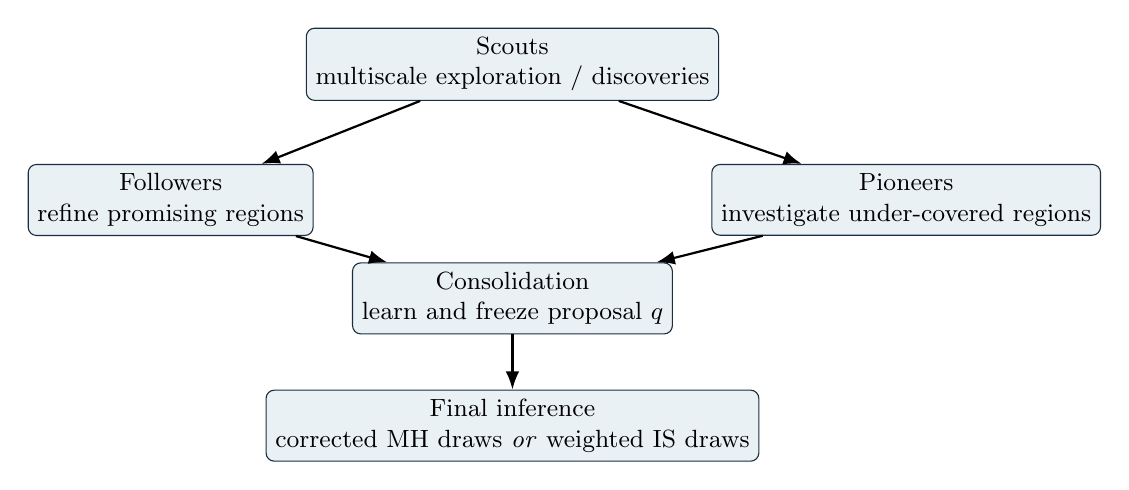
\begin{tikzpicture}[>=Latex,node distance=0.55cm and 1.0cm, every node/.style={font=\small},b/.style={draw=ink,rounded corners=3pt,align=center,minimum width=3.3cm,minimum height=0.8cm,fill=soft}]
\node[b] (scout) {Scouts\\multiscale exploration / discoveries};
\node[b,below left=0.8cm and -0.1cm of scout] (follow) {Followers\\refine promising regions};
\node[b,below right=0.8cm and -0.1cm of scout] (pioneer) {Pioneers\\investigate under-covered regions};
\node[b,below=2.05cm of scout] (freeze) {Consolidation\\learn and freeze proposal \(q\)};
\node[b,below=0.7cm of freeze] (final) {Final inference\\corrected MH draws \emph{or} weighted IS draws};
\draw[->,thick] (scout)--(follow);
\draw[->,thick] (scout)--(pioneer);
\draw[->,thick] (follow)--(freeze);
\draw[->,thick] (pioneer)--(freeze);
\draw[->,thick] (freeze)--(final);
\end{tikzpicture}
\end{center}
The proposed advantage is not a new universal Markov transition: it is improved \emph{allocation of exploration and information transfer}. The stages must be understood separately. Scouts may use broad proposals, temperature changes, restarts, or repulsion. These states can be useful in proposal construction while being unsuitable for posterior estimation. Followers explore credible local regions; pioneers deliberately favor directions or regions with inadequate coverage. The final phase is responsible for valid posterior inference.

\section{Mathematical separation: discovery versus inference}
\subsection{A frozen proposal with corrected Metropolis--Hastings}
Let the exploratory phases construct a normalized, evaluable proposal \(q(x)\), often a Gaussian mixture with a broad defensive component. After proposal construction stops, an independence proposal \(Y\sim q\) is accepted from the current state \(X=x\) with probability
\begin{equation}\label{eq:imh}
\alpha_{\mathrm{ind}}(x,y)=\min\left\{1,\frac{\widetilde\pi(y)q(x)}{\widetilde\pi(x)q(y)}\right\}.
\end{equation}
A separate symmetric local random-walk proposal uses
\(\alpha_{\mathrm{loc}}(x,y)=\min\{1,\widetilde\pi(y)/\widetilde\pi(x)\}\).
With fixed, state-independent mixing probabilities, a mixture of these target-invariant kernels remains target-invariant. \textbf{Correct stationary distribution is not equivalent to rapid mixing or demonstrated convergence.} A single final chain may remain trapped even if earlier explorers reached other important regions. Adaptive steps during final warmup must be frozen before retained draws are interpreted under a fixed-kernel argument; see standard MCMC and adaptive-MCMC references \citep{robert2004,haario2001,roberts2007}.

\subsection{An alternative final estimator: importance sampling}
In a later \emph{importance consolidation} branch, the final stage generates fresh independent \(X_i\sim q\), then computes
\begin{equation}\label{eq:is}
w_i=\frac{\widetilde\pi(X_i)}{q(X_i)},\qquad
\widehat{\mathbb E_\pi[h]}=\frac{\sum_{i=1}^n w_i h(X_i)}{\sum_{i=1}^n w_i},\qquad
\mathrm{ESS}_{\mathrm{IS}}=\frac{(\sum_i w_i)^2}{\sum_i w_i^2}.
\end{equation}
These are \emph{weighted observations}, not draws from the final MH chain, and their ESS is not interchangeable with autocorrelation-based MCMC ESS. Broad support of \(q\) is essential but does not by itself prevent catastrophic finite-sample importance-weight concentration.

\subsection{Experimental fairness}
Most simulation scripts explicitly budget the number of evaluations of \(\log\widetilde\pi\), including screening candidate starts, initialization, exploration and final inference. That is appropriate for one notion of computational fairness but does \emph{not} equalize CPU wall time, matrix factorization, proposal density evaluation, effective retained sample size, or implementation quality. Scores against known mixture components or analytic posterior references are used \emph{post hoc}; they must never be fed to a sampler.

\section{Development chronology and hypotheses}
\small
\begin{longtable}{p{0.205\linewidth}p{0.425\linewidth}p{0.285\linewidth}}
\toprule
\textbf{Study or branch} & \textbf{Methodological question} & \textbf{Evidence and current status}\\
\midrule\endfirsthead
\toprule\textbf{Study or branch} & \textbf{Methodological question} & \textbf{Evidence and current status}\\\midrule\endhead
Early formation and Experiment 2 & Do pioneer starts outperform random starts or follower-only starts under identical exploration budgets? & 100-replicate saved summary; randomized variant was competitive or better.\\
Experiment 3 & Does targeting \emph{unexplored} plausible locations help versus novelty, density, diversity, random and adaptive-mixture controls? & 100-replicate saved results; moderate average advantages with uncertainty.\\
Experiment 4 & Do the heuristics improve more consequential posterior functionals and mode reporting? & 100-replicate saved summary; FLOCK-Novelty close to adaptive-mixture MH, followers worse.\\
Map / MapMerge; Experiment 5 & Can location/covariance maps reduce redundant exploration and resolve rare modes in a six-component 10D mixture? & 3-replicate smoke and first 25 completed replicates visible in console log; no verified complete 100-replicate result.\\
Orthogonal / SoftOrth & Can covariance eigendirections direct pioneers into neglected directions? & 2-replicate scenario summaries available; small, unstable basis for inference.\\
Dog Walker / repulsion & Can multiple mutually repelling explorers improve coverage before corrected final sampling? & Code and theta-squared diagnostic table; repulsion has a different exploration target, not posterior draws.\\
FLOCK--AM formation controls & Do role assignments add value when final kernels and proposal machinery are matched to staged AM? & Standalone R scripts and some saved pilots; archived full scores not fully accessible here.\\
Hard multimodal tests & Does the strategy survive ridges, funnels, label switching, and consequential modes? & Benchmark scripts and ZIP archives found; underlying ZIP result tables were not retrievable in this export.\\
Importance consolidation & Do role-specialized explorers produce a better frozen proposal for self-normalized importance sampling? & Reported 10-replicate 5D pilot favors roles on several metrics; archive cannot be independently rechecked here.\\
\bottomrule
\end{longtable}
\normalsize
The chronology represents \emph{experiments explored}, not a claim that each script improved on the prior one, nor that every branch has passed equivalent validation.

\section{Targets and metrics}
\subsection{Known mixtures}
The early 5D experiments use four Gaussian mixture components with weights \((0.45,0.30,0.20,0.05)\), separated locations, and heterogeneous scales; the 5\% narrow component is deliberately difficult. Experiment 5 instead uses a correlated \(10\)-dimensional mixture with six component weights $0.30,0.25,0.20,$ and $0.15,0.08,0.02$, including overlapping pairs. The importance-consolidation pilot uses a different four-component family with weights \((0.44,0.30,0.21,0.05)\). These are \emph{distinct targets}: their RMSE values should not be compared as if on one common scale.

\subsection{Posterior targets arising from statistical models}
The additional benchmark scripts include a two-test diagnostic latent class posterior with disease-label ambiguity, a nearly collinear 40-coefficient regression with sparse mixture priors, a product ridge with sign branches, a weak-signal hierarchical funnel, a label-switching three-component mixture, and a theta-squared posterior illustrating two sign modes. A later hard-target script adds a mode-sign ambiguity with predictive consequences. Label-switched configurations and conditional identifiability failures are not interchangeable with physically distinct posterior explanations.

Metrics include errors in posterior means, component mass or event probabilities, covariance matrices, marginal credible interval endpoints, group occupancy, mode transitions, acceptance and time. For each scenario, the primary scientific estimand should be stated \emph{before} comparing algorithms; performance on a convenient surrogate such as mean RMSE is not automatically performance on consequential posterior decisions.

\section{Observed results: original summary tables}
\subsection{Experiment 2: initial ablation, 100 replicates}
\begin{table}[H]\centering\small
\begin{tabular}{lrrrr}
\toprule
Method & Mean RMSE & Weight L1 & Rare visit rate & Mean acceptance\\
\midrule
FLOCK (targeted) & 2.192 & 0.760 & 0.03 & 0.352\\
FLOCK-Followers & 2.557 & 0.868 & 0.03 & 0.380\\
FLOCK-Random & \textbf{2.032} & \textbf{0.710} & 0.03 & 0.329\\
\bottomrule
\end{tabular}
\caption{Direct transcription (rounded) from \protect\path{flock_experiment_2_summary.csv}. Each method has 100 reported replications. Lower RMSE/L1 is better; rare visitation is a diagnostic, not a guarantee of accurate mass allocation.}
\end{table}
Contrary to the initial hope, the randomized-start ablation did \emph{not} perform worse on these average error metrics. The targeted FLOCK comparison with random gave a mean RMSE difference \(0.160\), with reported bootstrap interval \([-0.123,0.450]\). This result directly motivated more controlled candidate-selection comparisons.

\subsection{Experiment 3: pioneer policy, 100 replicates}
\begin{table}[H]\centering\small
\begin{tabular}{lrrr}
\toprule
Method & Mean RMSE & Mean weight L1 & Rare detection\\
\midrule
FLOCK-Unexplored & \textbf{1.901} & \textbf{0.669} & 0.04\\
AdaptiveMixtureMH & 2.059 & 0.706 & 0.01\\
FLOCK-Novelty & 2.055 & 0.720 & 0.03\\
FLOCK-Random & 2.106 & 0.724 & 0.03\\
FLOCK-Diversity & 2.135 & 0.739 & 0.02\\
FLOCK-Density & 2.141 & 0.752 & 0.03\\
FLOCK-Followers & 2.485 & 0.845 & 0.03\\
\bottomrule
\end{tabular}
\caption{Saved \protect\path{flock_experiment_3_summary.csv} (100 replicates per method); source code \protect\path{flock_experiment_3.R}. Component diagnostic references were not used by the sampler.}
\end{table}
\begin{figure}[H]\centering\IfFileExists{figures/exp3_rmse.png}{\includegraphics[width=0.92\linewidth]{figures/exp3_rmse.png}}{\fbox{\parbox{0.85\linewidth}{\centering Figure file missing: \texttt{exp3\_rmse.png}.\\ Add the original PNG from the Overleaf project to restore this plot.}}}\caption{Replotted saved mean RMSE values for Experiment 3. Error bars are intentionally omitted; assess the paired uncertainty in text and in the CSV.}\end{figure}
The paired mean difference \(\mathrm{RMSE}_{\mathrm{Unexplored}}-\mathrm{RMSE}_{\mathrm{AdaptiveMixtureMH}}=-0.157\) had reported bootstrap interval \([-0.500,0.207]\) and a 57\% fraction of replicate wins. It is therefore \textbf{not convincing evidence of consistent superiority}. Rare mode detection improved from 1\% to 4\%, but both rates were poor, with estimated rare mass far below the true 5\% mass.

\subsection{Experiment 4: functional performance, 100 replicates}
\begin{table}[H]\centering\small
\begin{tabular}{lrr}
\toprule
Method & Mean functional RMSE & Mean label error\\
\midrule
FLOCK-Novelty & \textbf{0.01477} & \textbf{0.02289}\\
AdaptiveMixtureMH & 0.01525 & 0.02474\\
FLOCK-Unexplored & 0.01769 & 0.02837\\
SAChES-inspired & 0.04865 & 0.08007\\
FLOCK-Followers & 0.05126 & 0.11608\\
RWMH (four chains) & 0.07112 & 0.16750\\
\bottomrule
\end{tabular}
\caption{Saved \protect\path{flock_experiment_4_summary.csv}, each with 100 replications. The metric definitions here differ from the five-dimensional RMSE in Experiment 3.}
\end{table}
\begin{figure}[H]\centering\IfFileExists{figures/exp4_rmse.png}{\includegraphics[width=0.92\linewidth]{figures/exp4_rmse.png}}{\fbox{\parbox{0.85\linewidth}{\centering Figure file missing: \texttt{exp4\_rmse.png}.\\ Add the original PNG from the Overleaf project to restore this plot.}}}\caption{Observed average functional errors for Experiment 4. Do not infer a significant difference from bar length alone.}\end{figure}
FLOCK-Novelty was close to AdaptiveMixtureMH in mean functional RMSE (approximately 0.0148 vs 0.0152). The saved paired table uses FLOCK-Unexplored as one reference method; it also demonstrates that method rankings vary by metric. Neither the strong loss for follower-only exploration nor the close two-method comparison supports a universal role advantage.

\subsection{Orthogonal exploration: preliminary scenario comparisons}
A separately saved \protect\path{method_summary.csv} contains only \(n=2\) runs for each of three prototype scenarios, so these are \textbf{descriptive code-check results only}. For ProductRidge, mean error was 0.161 for FLOCK-Novelty, 0.283 for AdaptiveMetropolis, and 0.557 for FLOCK-Orthogonal; for WeakSignalFunnel it was 0.062 for Orthogonal, 0.126 for Novelty, and 0.246 for AdaptiveMetropolis; for ThreeComponentMixture it was 0.074 for AdaptiveMetropolis, 0.148 for Novelty, and 0.254 for Orthogonal. The sign reversals are informative about sensitivity to target geometry, not proof of any preferred variant.

\subsection{Theta-squared posterior: how final-chain accuracy can differ}
The saved \protect\path{reference_summary.csv} gives an exact reference posterior mean of 1.712 and posterior probability \(P(\theta>0)=0.789\) for the theta-squared example. The historical \protect\path{method_posterior_summaries.csv} compares methods at 96,000 target calls each. Some illustrative posterior mean estimates were FLOCK-Novelty 1.701, AdaptiveMixtureMH 1.762, DogWalker90 1.681, and RandomWalkMH 0.001. This illustrates the enormous influence of mode mixing on a non-invariant estimand. It is a single benchmark configuration: the full variance across independent repetitions is not established by this table. A pseudo-\(\widehat R\) near 1 is no substitute for comparing all chains against known nontrivial modes; the recorded independent RWMH chains had a very large classical \(\widehat R\) around 64.

\subsection{Experiment 5: 10D six-component Gaussian mixture}
\textbf{Smoke test.} In three replicates with \(B=5{,}000\) counted target calls, mean RMSE was 0.712 for FLOCK-Unexplored, 0.719 for AdaptiveMixtureMH, 0.720 for Map and MapMerge, 0.844 for RWMH, and 1.111 for Novelty. The recorded rare-core discovery rate was zero for \emph{all} methods. Smoke results are for debugging, not ranking.

\textbf{Visible full-log subset.} The accompanying console log reports that a run was initiated with \(100\) replicates and \(B=100{,}000\) evaluations per method; the accessible excerpt contains \emph{25 fully observed replicate blocks} and only part of replicate 26. We therefore summarize \(n=25\) rather than asserting that all 100 completed or that their results were recovered:
\begin{table}[H]\centering\small
\begin{tabular}{lrrr}
\toprule
Method & Mean RMSE & Median RMSE & Mean mass L1\\
\midrule
FLOCK-Novelty & \textbf{0.391} & 0.118 & \textbf{0.239}\\
ParallelTempering & 0.420 & 0.313 & 0.262\\
AdaptiveMixtureMH & 0.491 & \textbf{0.095} & 0.322\\
FLOCK-Unexplored & 0.546 & 0.133 & 0.337\\
FLOCK-Map & 0.550 & 0.123 & 0.323\\
FLOCK-MapMerge & 0.550 & 0.123 & 0.323\\
RWMH (four chains) & 1.399 & 1.188 & 0.804\\
SAChES-inspired & 1.891 & 1.897 & 1.033\\
\bottomrule
\end{tabular}
\caption{Recalculated from the first 25 complete visible replicates in \protect\path{experiment5_console_log_excerpt.txt}; not the complete advertised 100-replicate result.}
\end{table}
\begin{figure}[H]\centering\IfFileExists{figures/exp5_partial_rmse.png}{\includegraphics[width=0.92\linewidth]{figures/exp5_partial_rmse.png}}{\fbox{\parbox{0.85\linewidth}{\centering Figure file missing: \texttt{exp5\_partial\_rmse.png}.\\ Add the original PNG from the Overleaf project to restore this plot.}}}\caption{The 10D benchmark from the visible log subset. The Novelty--AdaptiveMixture mean difference of \(-0.100\) coexists with a Novelty win rate of only 11/25; heavy tails matter.}\end{figure}
Across these 25 paired replicates, FLOCK-Novelty had a lower RMSE than AdaptiveMixtureMH in only 11 runs (44\%), despite its lower mean error. Map and MapMerge yielded identical mean errors throughout the visible completed subset; this alone does not demonstrate that their internal maps or merging logic were identical. Complete archive audits and more replicates are needed.

\subsection{Importance-weighted consolidation: reported 5D pilot}
A later redesign asked whether the roles are more useful for \emph{learning a frozen importance proposal} than for a single terminal MH chain. A ten-replicate pilot with \(B=12{,}000\) target evaluations reportedly gave:
\begin{table}[H]\centering\small
\begin{tabular}{lrrrrr}
\toprule
Method & Mean RMSE & Mass L1 & Cov. err. & IS ESS & Time (s)\\
\midrule
FLOCK-Roles & 0.204 & 0.088 & 0.074 & 237 & 1.06\\
Undirected-Matched & 0.325 & 0.139 & 0.104 & 147 & 1.04\\
\bottomrule
\end{tabular}
\caption{\textbf{Previously reported, not archive-verified here.} The original \protect\path{flock_importance_5d_pilot_B12000.zip} was located in the user's Library but its raw contents could not be extracted in this export. Values are retained in \protect\path{importance_pilot_reported_prior_analysis_UNVERIFIED.csv} pending re-check.}
\end{table}
The earlier paired analysis reported FLOCK-Roles winning 7/10 RMSE comparisons; the paired RMSE difference interval \([-0.296,0.016]\) included zero. Other reported metrics (mass L1, covariance and interval endpoints) were more favorable, but the sample size was small. The result is promising \emph{for importance-weighted approximation under this target and control}, not validation of the original final-chain sampler.

\section{What failed, remained uncertain, or changed direction}
\begin{enumerate}[leftmargin=*]
\item \textbf{Directed starts were not reliably better.} The earliest 100-replicate random-start ablation beat the targeted baseline on average RMSE and L1, and the Unexplored/AdaptiveMixture comparison had substantial uncertainty.
\item \textbf{A lone final chain can discard information.} Earlier stages may have discovered modes that are absent from the final chain. A final chain cannot be forced to visit specific posterior regions by an uncorrected rule without changing its stationary law.
\item \textbf{Higher dimension changes the geometry.} Adaptive Metropolis and undirected controls can be strong on correlated targets. Covariance-based orthogonal exploration is expensive and does not necessarily solve low-probability-mode discovery.
\item \textbf{Exploration is not inference.} Temperature changes, novelty penalties, repulsion, and restarts can be useful in scouting but do not make exploratory samples posterior samples.
\item \textbf{Mode count is not accuracy.} Gaussian-mixture components can overlap, label permutations can represent the same scientific state, and component-core discovery can coexist with badly wrong mass estimates.
\item \textbf{The proposal map did not show a clear benefit in the accessible 10D subset.} A separate audit of merge counts, local acceptance, and final transitions is needed to identify whether the design was ineffective or inactive.
\item \textbf{Importance consolidation is conceptually different.} The redesign avoids the need for one final chain to traverse every mode, but introduces finite-sample importance weight degeneracy and requires a well-supported proposal density.
\item \textbf{No established convergence theorem or general novelty claim.} Controlled comparisons isolate some mechanisms, not a new universally superior MCMC law. Code has not been executed afresh while preparing this notebook.
\end{enumerate}
A separate, ultimately paused idea considered using explorer/follower disagreement to test posterior model fit. It did not lead to a justified null distribution or a calibrated goodness-of-fit method, and should \emph{not} be represented as part of the established FLOCK sampler.

\section{Reproducibility and code architecture}
\subsection{What the repository contains}
\begin{itemize}
\item \protect\path{scripts/}: original standalone R benchmark source snapshots, including experiments 2--5, orthogonal and SoftOrth extensions, controlled AM comparisons, Dog Walker, hard targets, and importance consolidation.
\item \protect\path{notes/}: source-specific documentation and experiment settings copied from the original research notes.
\item \protect\path{data/}: recovered CSV summaries and per-replicate records, a visible console-log excerpt, and a clearly marked table of \emph{unverified prior reports}.
\item \protect\path{figures/}: plots regenerated \emph{only} from recovered aggregate tables and the visible console-log subset.
\item \protect\path{analysis/}: scripts for validating tabular provenance and reproducing plots; see README for commands.
\end{itemize}
The scripts are historical research snapshots; several have their own global functions and output conventions. \emph{Do not source all scripts into one R session.} No full R runtime check was possible in the environment assembling this document. Start with each script's smoke-mode command and run in a fresh R session and output directory.

\subsection{Recommended minimal reproduction}
\begin{lstlisting}
# From the repository root, in a fresh R session:
setwd('scripts')
Sys.unsetenv(c('REPS','BUDGET','OUTDIR','METHODS'))
Sys.setenv(REPS='5', BUDGET='20000')
source('flock_experiment_3.R')
# Compare newly generated outputs to data/ only after
# checking target, seeds, method set, and script version.
\end{lstlisting}
For Experiment 5, use its documented \protect\path{RUN_MODE=smoke} setting first. For importance consolidation, use its 2D smoke test, then the 5D pilot only if the invariance/weight checks pass. Consult the per-script README before changing environment variables, which may override mode defaults. A comprehensive rerun should record Git commit, R version, seed, target definition, \(B\), actual target calls, elapsed time, number of retained final samples, and convergence diagnostics.

\subsection{Predeclared decision checklist for a future formal study}
\begin{enumerate}
\item Choose a consequential posterior estimand \(h(\theta)\) and define a reference computed independently from the algorithm.
\item Distinguish whole-method comparisons from controlled ablations (same scouts, candidate sets, budget, kernels, and final estimator).
\item Benchmark with both fixed target-call counts and elapsed time; compare uncertainty across many paired random replicates.
\item Report false assurance: missed regions discovered earlier, between-run variation, label switches, poor within-chain transitions, global proposal acceptance, MCMC ESS, and IS weight concentration.
\item Separate exploratory diagnostics, valid final MH retained draws, and weighted IS outcomes in both filenames and figures.
\item Include failures and counterexamples. Do not promote a variant based solely on its best scenario or a post hoc selected metric.
\end{enumerate}

\section{Conclusions and research status}
The evidence supports a narrow and useful conclusion: role-specialized exploration is a \emph{testable design hypothesis} that sometimes improves posterior approximation under constrained target-evaluation budgets, especially when it learns a useful proposal or finds otherwise neglected regions. However, randomized exploratory starts and adaptive Metropolis often remained competitive, gains were sensitive to target geometry and metric, and the single-final-chain consolidation stage was a recurring limitation. The later importance-weighted variant has a distinct promise but cannot retroactively validate the MCMC approach. The appropriate status is \emph{exploratory, archived, awaiting reproducible confirmatory tests}, not a finished new sampling algorithm.

\section*{Source provenance and limits of this reconstruction}
\addcontentsline{toc}{section}{Source provenance and limits of this reconstruction}
\textbf{Directly checked here:} retrieved source R text, the original experiment 2--4 and orthogonal benchmark CSV summaries, theta-squared posterior summaries, and the first 25 complete visible blocks of an Experiment 5 console transcript. Recomputed tables and figures are included in the repository.\par
\textbf{Previously discussed but not rechecked:} the 5D importance-consolidation pilot values and selected qualitative conclusions about later hard benchmarks. These are marked accordingly. The user Library also contains multiple ZIP result archives, including the B=12,000 importance pilot, hard multimodal B=20,000 pilot, and AM/final/orthogonal pilots; the ZIP bytes were not accessible from this session and were \emph{not} silently replaced with invented results. No new FLOCK simulation was executed for this document.\par
\textbf{Public sharing:} prior research discussions treated this formation as private. If posting on GitHub, review whether to use a private repository first. Publishing code or the notebook makes the underlying method public.

\begin{thebibliography}{9}
\bibitem[Haario et al.(2001)]{haario2001}
Haario, H., Saksman, E., and Tamminen, J. (2001).
An adaptive Metropolis algorithm. \emph{Bernoulli}, 7(2), 223--242.
\url{https://doi.org/10.2307/3318737}.
\bibitem[Roberts and Rosenthal(2007)]{roberts2007}
Roberts, G. O. and Rosenthal, J. S. (2007).
Coupling and ergodicity of adaptive Markov chain Monte Carlo algorithms.
\emph{Journal of Applied Probability}, 44(2), 458--475.
\url{https://doi.org/10.1239/jap/1183667414}.
\bibitem[Robert and Casella(2004)]{robert2004}
Robert, C. P. and Casella, G. (2004).
\emph{Monte Carlo Statistical Methods}, 2nd ed., Springer.
\url{https://doi.org/10.1007/978-1-4757-4145-2}.
\end{thebibliography}
\end{document}